%!TEX root = ../thesis.tex

\chapter{Introduction}
\label{ch:intro}
\section{Background and Motivation}
The most important asset a company possesses in this day and age is its data and with increasing volume and awareness the challenges around data storage, security, and consumption are also growing exponentially. Some organizations either have already shifted towards a cloud or hybrid architecture and some are in the process of this shift. The move to the cloud offers a flexible and robust solution for data storage as well as access control to the data through some kind of Role-Based Access Control (RBAC).

\bigskip
Many organizations, often competitors, possess datasets with similar information. These organizations may be interested in sharing insights from their data but are reluctant to expose their data and transfer ownership to others. The goal of such knowledge sharing would be to drive the research of the entire industry but concerns over data privacy and ownership hinder such collaboration.

\bigskip
The traditional approach towards complex analytical algorithms on some datasets involve transferring data, which may be originating from several sources, close to the compute resources, and then running the algorithms or training an AI model. But the approach becomes impractical when multiple organizations become involved and data sharing becomes complicated owing to regulations and privacy.

\bigskip
An approach garnering more and more focus is to move the computation closer to the data residence; solving most of the storage and security concerns. One concern, however, would be to develop the expertise in writing distributed code which could be expensive and time-consuming.

\bigskip
We propose a solution allowing orchestration of complex workflows where each job in the workflow consumes some data from one or multiple sources and results from individual jobs can be compiled when the workflow finishes. Such a design would allow organizations to share their data for consumption by algorithms while still maintaining the ownership of the data. And also eliminating the need to invest heavily into developing knowledge of writing distributed algorithms for utilization of data from multiple sources.


\section{Objectives}
The aim of this thesis project is to develop a proof of concept that will enable untrusting organizations to share their datasets while maintaining ownership and access control over the data. The system would allow users to write code and complex workflows to consume datasets from multiple sources without exposing the data itself to the users. The integration of this thesis with \cite{nft-thesis}, in the future, will help in proving ownership of datasets and computed results as Non-Fungible Tokens.

\begin{figure}
    \centering
    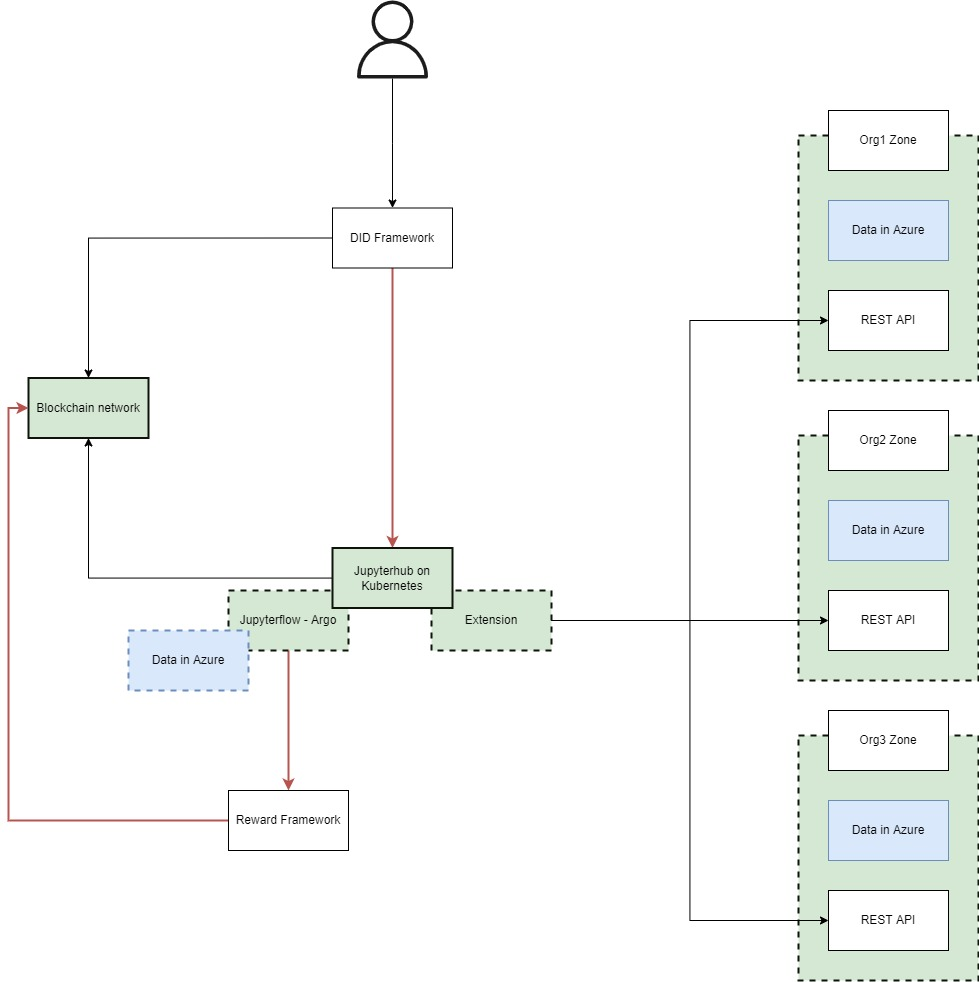
\includegraphics[width=14cm,keepaspectratio]{photos/Overview.jpg}
    \caption{Architecture of the overarching MVP that this thesis is a part of and the scope of the thesis}
    \label{fig:overview}
\end{figure}

\bigskip
The overarching Minimum Viable Product (this thesis in integration with Distributed Identity - DID and Data \& Results as NFTs) will allow for workflow design and development with access control of the entire system through DID and incentivization for contribution to the consortium through NFTs. The figure \ref{fig:overview} illustrates the architecture of the complete MVP. However, the scope of this thesis is highlighted by the green portions and is solely focused on the system for workflow design and data consumption. The DID and Reward Framework along with integrations highlighted in red fall outside the scope of this thesis.

\bigskip
The scope of this project comprises of following parts:
\begin{itemize}
    \item Establishing a blockchain network for containing meta-data of available datasets and a log of lease history of the data along with the chain code for committing the transaction to the ledger. The blockchain is constructed on Hyperledger Fabric.
    \item A REST API for keeping track of encryption keys in a MySQL Database and invoking the chain-code for respective requests.
    \item JupyterHub on a Kubernetes cluster where each organization can contribute nodes that will host Jupyter notebooks for users and act as an orchestrator for the entire system allowing design and execution for the workflows.
    \item An extension for JupyterHub that the users can utilize to explore and start work with a dataset.
    \item Extending JupyterFlow to mount Persistent Volumes on Kubernetes, create Persistent Volume Claims and trigger Argo Workflows on the cluster to run the user's code in a containerized form.
\end{itemize}

\section{Approach and Contributions}
The first component of our proposed system is to set up a blockchain network in Hyperledger where metadata of the datasets will be hosted. The idea behind using a blockchain is to enable organizations complete control over the information without trusting a third party as the maintainer of the system. The ledger keeps a track of all the datasets available from different organizations and a ledger of which organizations are using or have used the data. And the chaincode that could read and modify the state of the ledger. 

\bigskip
The next component is a REST API acting as the gateway between the blockchain and JupyterHub. We develop the API that responds to calls from the JupyterHub, does the validations on the requests, and invokes the corresponding chaincode. The API also stores and keeps track of the keys used to encrypt the sensitive information before committing to the blockchain. This API is going to be internal to the organization to keep the security of the keys integral.

\bigskip
The next key to the solution is the development of a custom Data Explorer extension for JupyterHub that will be interacting with the REST API and will be the interface for exploring and leasing the datasets as well as some admin operations for the maintenance of datasets. In this thesis the admin portion is visible to all however the integration with DID will enable fine-grain access control over the system. On triggering the lease of a dataset, a transaction is submitted to the blockchain, then a folder structure of the data is created in the user's JupyterHub environment to allow them to write code for the dataset and finally make the metadata ready for JupyterFlow to use by reading un-encrypted information vital for mounting the dataset on Kubernetes.

\bigskip
Finally, we fork and further develop the JupyterFlow \footnote{\url{https://github.com/hongkunyoo/jupyterflow}} to add the functionality enabling the mounting of data as persistent volumes in Kubernetes. The data can either be from a node in the Kubernetes cluster that the organization owns or from an Azure Fileshare. JupyterFlow then reads the information from the extension and creates persistent volume and persistent volume claims, generates an Argo workflow from the provided workflow YAML written by the user, and triggers the workflow to run.

\bigskip
Additionally, during the setup phase, we create a Kubernetes service account and set the token in the docker image where we also install the data explorer extension, our custom JupyterFlow, and some other dependencies. This docker image is used to spin up instances of Jupyter whenever a user logs in to the JupyterHub.

\section{Outline}

\subsection{Chapter 2 - Related Work}
This chapter presents some of the related work for this thesis and discusses the differences in our approach in comparison to the previous research and inspirations for some of the ideas in our thesis.

\subsection{Chapter 3 - Background}
In chapter three we present some background knowledge about the tools and technologies we have chosen for the development of our solution and discuss the reasoning behind the tools we have chosen.

\subsection{Chapter 4 - Approach}
In this chapter, we present and discuss our approach to developing the solution. We describe in detail how we use the different technologies and discuss the architecture of the proposed system. 

\subsection{Chapter 5 - Experiment and Demo}
Here we demonstrate how we have set up the test environment and the experiments we conducted on our system.

\subsection{Chapter 6 - Conclusions and Future Work}
Finally, we conclude our work, summarize the project and discuss the future directions for the project.